\def\W{\Omega}
\def\w{\omega}
\def\mycap{\,\cap\,}
\def\mycup{\,\cup\,}

\def\sc{1cm}
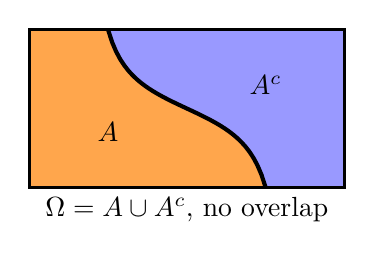
\begin{tikzpicture}[x=\sc,y=\sc]
% graph
\draw [fill=blue!40!white] (-2,-1) rectangle (2,1);
\begin{scope}
% This curve is normalize to go from -1,-1 to 1,1. 
%It divides the rectangle in two
\clip plot [domain=-1:1,samples=40] 
        ({\x},{tan(-1.2*\x r)/2.5722}) -- (-2,-1) -- (-2,1) -- cycle;
% the clip region will keep the shading within bounds
\draw [fill=orange!70!white] (-2,-1) rectangle (2,1);
\end{scope}
\draw [line width=1.5, domain=-1:1,samples=40] plot ({\x},{tan(-1.2*\x r)/2.5722});
\draw [line width=1.2] (-2,-1) rectangle (2,1);
\node at (-1,-.3) {$A$};
\node at (1,.3) {$A^c$};
\node at (0,-1) [below] {$\W = A \cup A^c$, no overlap};
\end{tikzpicture}
